\documentclass[10pt]{article}
\usepackage[letterpaper,margin=1in]{geometry}
\usepackage{times}
\usepackage[T1]{fontenc}
\usepackage{amsmath,amssymb,amsthm}
\usepackage{booktabs}
\usepackage{graphicx}
\usepackage[table]{xcolor}
\usepackage{colortbl}
\usepackage[numbers,sort&compress]{natbib}
\usepackage[colorlinks,allcolors=blue!50!black]{hyperref}
\usepackage[expansion=false]{microtype}   % no font expansion: body text stays at exactly 10 pt (RECOMB minimum)
\usepackage{placeins}
\renewenvironment{abstract}{\begin{center}\textbf{Abstract}\end{center}\noindent\ignorespaces}{\par}   % article's abstract is 9 pt
\renewcommand{\topfraction}{0.9}
\renewcommand{\bottomfraction}{0.8}
\renewcommand{\textfraction}{0.07}
\renewcommand{\floatpagefraction}{0.8}
\setcounter{topnumber}{3}
\setcounter{totalnumber}{4}

\definecolor{ours}{RGB}{228,243,242}
\newcommand{\cad}{CellAsDistribution}
\newcommand{\tbd}[1]{{\color{red}\textbf{TBD}\,(#1)}}
\newcommand{\todo}[1]{{\color{red}[TODO: #1]}}
\newcommand{\cadc}{CAD}
\newcommand{\cadf}{CAD-P}
\newcommand{\cadn}{CAD-N}
\newcommand{\cadr}{CAD-R}
% Backbone of the decision language model (main model; Qwen3.5-0.8B is the second backbone).
\newcommand{\backbone}{C2S-Scale-Gemma-2-2B}
\newcommand{\autoinput}[1]{\IfFileExists{#1}{\input{#1}}{\todo{missing \detokenize{#1}}}}
\newtheorem{proposition}{Proposition}
% sentence-style headings: break between words, never hyphenate (article's sizes and spacing otherwise unchanged)
\makeatletter
\renewcommand\section{\@startsection{section}{1}{\z@}{-3.5ex \@plus -1ex \@minus -.2ex}{2.3ex \@plus.2ex}{\normalfont\Large\bfseries\raggedright\hyphenpenalty=10000}}
\renewcommand\subsection{\@startsection{subsection}{2}{\z@}{-3.25ex\@plus -1ex \@minus -.2ex}{1.5ex \@plus .2ex}{\normalfont\large\bfseries\raggedright\hyphenpenalty=10000}}
\makeatother

\title{Why Generate a Sentence? A Decision Language Model for Modeling Single-Cell Composition}
\author{Anonymous submission}
\date{}

\begin{document}
% Title page (title, authors, abstract) is the additional page permitted by the call; the 10-page body starts on page 1.
\pagenumbering{gobble}
\maketitle
\thispagestyle{empty}

\begin{abstract}
Predicting the transcriptome of cells in unmeasured conditions, such as unseen cell types or genetic perturbations, is central to building virtual cells, and language models promise to condition these predictions on text. Current single-cell language models, however, write each cell as a sentence of gene names ranked by expression and generate it token by token: their output must be heuristically mapped back to counts, lacks a count likelihood, and is slow to decode. We introduce CellAsDistribution, which represents a cell on a fixed gene panel as the probability distribution of its transcript counts. A softmax decision head over the panel on a condition encoder returns this distribution from a text prompt in one forward pass, scoring every method by the exact multinomial likelihood of held-out counts. On held-out CRISPRa perturbations in K562, CellAsDistribution outperforms Cell2Sentence fine-tuned on the same backbone by 0.10 nats per UMI, raises correlation on downstream differentially expressed genes from 0.56 to 0.77, decodes 90 to 540 times faster, and matches additive composition of known effects. Pre-registered controls show that this gain comes from the distribution output rather than language-model knowledge, and that no learned representation predicts responses to genes never perturbed in training; on human PBMC, a backbone pretrained on cell sentences generates unseen cell types from their names. By placing sentence models, count models, and simple baselines on one proper scale, our decision-native interface separates how a cell is represented from what its encoder knows.
\end{abstract}
\clearpage
\pagenumbering{arabic}

\section{Introduction}
Predicting the transcriptional state of cells in an unmeasured condition, such as a cell type in a new donor or a genetic perturbation, is the central task of the ``virtual cell'' program~\citep{bunne2024virtualcell}.
A useful generator must say not only which genes change but how a cell's transcripts are distributed over genes, and it must be judged by the probability it assigns to cells it has not seen.
Language models are attractive for this task because a condition can be stated in text: Cell2Sentence (C2S) writes each cell as a sentence of gene names ordered by decreasing expression and fine-tunes a pretrained language model on these sentences~\citep{levine2024cell2sentence,rizvi2025c2sscale}.
The model then generates a cell token by token, and its output is text: a ranked list of names that must be mapped back to expression before it can be compared with counts.

We ask a simple question: why generate a sentence at all?
On a fixed panel of $G$ genes, the counts of a cell divided by their sum form a probability distribution over the panel, and together with the library size they reproduce the counts exactly (Proposition~\ref{prop:repr}).
A \emph{decision language model} answers a prompt not with text but with a probability over a fixed set of options in one forward pass~\citep{unsloth_decision,typesafe2026jev}.
If the options are the genes of the panel, the answer \emph{is} a cell: the expected share of its transcripts that each gene contributes.
We call this framework \cad{} (Figure~\ref{fig:overview}).
Given a text state (a cell type, or a perturbation with an optional control cell), the model outputs a normalized gene distribution in a single pass; counts are sampled from this distribution, and the multinomial likelihood of held-out counts scores the model on the same scale as any other generator.
Because the output space is fixed, the condition encoder can be swapped: the same head can sit on a fine-tuned language model or on plain gene embeddings, allowing us to isolate what each component contributes.

\begin{figure}[t]
\centering
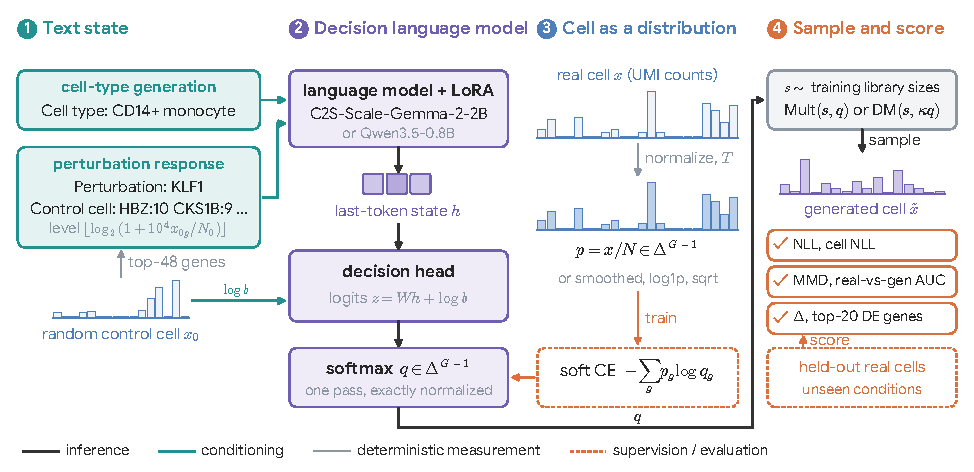
\includegraphics[width=\linewidth]{figs/fig1_method.pdf}
\caption{\textbf{A decision language model reads a text state and returns, in one forward pass, a distribution over a fixed gene panel; every method is scored with the same likelihood and sampler.} (1) The state is a prompt: a cell type, or a perturbation, optionally with a control cell $x_0$. (2) A LoRA-tuned language model encodes the prompt; a linear decision head on the last-token state, with an optional fixed log-prior $b$ (none, the training mean, or the smoothed control cell), gives one logit per gene, and a softmax gives $q$ on the simplex. (3) A real cell is the probability vector $p=x/N$ of its counts; training minimizes the cross-entropy between $p$ and $q$. (4) A shared sampler draws cells from $q$; held-out cells of unseen donors, perturbations, or cell types score the model.}
\label{fig:overview}
\end{figure}

Because this formulation is simple, its value must be established empirically, and we use it to dissect text-based cell generation along three questions.
\textbf{Interface (Section~\ref{sec:repr}).} Does generating the distribution directly beat generating a rank sentence on the same backbone and budget, and where does the sentence lose likelihood?
\textbf{Language model (Section~\ref{sec:lm}).} Does the fine-tuned language model matter, or would any encoder of the condition suffice?
\textbf{Biology (Sections~\ref{sec:pert}--\ref{sec:condgen}).} Does a better gene distribution yield better biology: the downstream response to a perturbation once the trivially induced target gene is set aside, the realism of single cells, and generalization to conditions never seen in training?
We answer these questions on human PBMC (generation for unseen donors and unseen cell types) and on the CRISPRa screen of Norman et al.\ in K562 (response to held-out perturbations), where simple baselines are known to be hard to beat~\citep{ahlmann2025deep,wei2026benchmark}.
Our contributions are:
\begin{enumerate}
\item \textbf{A decision-native framework for single cells.} A softmax decision head over a fixed gene panel, on a fine-tuned language model or on gene embeddings, returns a normalized gene composition in one pass with an exact multinomial score, placing sentence models, count models, and simple baselines on one proper scale (Section~\ref{sec:method}).
\item \textbf{Where sentence generation loses.} On the same backbone and budget, direct decoding gains $0.10$ nats per UMI over autoregressive C2S at $90$ to $540$ times lower decoding cost; rewriting real cells separates the loss of the published rank-to-count map from the loss of the ranks themselves, and re-decoding generated sentences shows that generation, not only the map, falls short (Section~\ref{sec:repr}).
\item \textbf{What the language model contributes, and the biological boundary.} Pre-registered controls show that the gain comes from the distribution output and that the language model's measured role is the text interface; under leakage-controlled splits, \cad{} matches additive composition of known effects on likelihood and on downstream differentially expressed genes, shrinks the induction of the targeted gene, generates unseen cell types from their names, and makes no gene-specific prediction for genes never perturbed in training (Sections~\ref{sec:lm}--\ref{sec:condgen}).
\end{enumerate}

\section{Related work}\label{sec:background}
\paragraph{Decision language models.}
A decision language model returns a probability over a bounded set of options for a typed question in a single pass instead of generating text to be parsed~\citep{typesafe2026jev,deusser2026jev}. The open implementation we build on attaches a classification head to the final hidden state of a pretrained model and trains it with the cross-entropy on soft targets~\citep{unsloth_decision}. The head itself is a standard softmax classifier; what is new here is choosing the genes of a panel as the options, so that the output distribution is a cell.

\paragraph{Cells as text and cell foundation models.}
Cell2Sentence fine-tunes language models on rank-ordered gene sentences and has been scaled to billions of parameters~\citep{levine2024cell2sentence,rizvi2025c2sscale}; its case for the representation is that expression is recovered from rank by a log-linear fit with high $R^2$. Other foundation models pretrain on expression tokens (scGPT, Geneformer)~\citep{cui2024scgpt,theodoris2023geneformer}, learn cell embeddings (UCE)~\citep{rosen2023uce}, or decode the whole profile from a bottleneck token (BMFM-RNA)~\citep{danziger2025bmfm}; none returns a normalized distribution from a text condition.

\paragraph{Count generators and perturbation predictors.}
scVI and scANVI decode gene frequencies inside a negative-binomial likelihood conditioned on latent states and labels~\citep{lopez2018scvi,xu2021scanvi}. Our output head uses the same parameterization (a softmax over genes, scaled by library size, optionally with gene-wise dispersion); what differs is its input, a text state read in one pass, which places sentence models, count models, and baselines on one common scale. scDiffusion samples cells with a conditional diffusion model~\citep{luo2024scdiffusion}, and the Gene Mover's Distance compares cells as distributions over genes~\citep{gmd2021}. Perturbation predictors such as scGen, CPA, GEARS, and State map a perturbation to an expression change~\citep{lotfollahi2019scgen,lotfollahi2023cpa,roohani2024gears,adduri2025state}, and population models learn copulas, flows, or transport between control and perturbed cells~\citep{wang2026poppert,yu2026scdfm,chen2026scale,han2026tempobridge,chi2025departures,jiang2026ocoot}. Independent benchmarks find that mean, additive, and linear baselines are hard to beat~\citep{ahlmann2025deep,wei2026benchmark} and that control-referenced metrics are inflated by systematic variation~\citep{vinas2025systema}; our main references are therefore the perturbed mean and additive composition.

\section{Decoding a cell as a gene distribution}\label{sec:method}
\subsection{A cell as a distribution over a fixed gene panel}\label{sec:why}
Let $x\in\mathbb{N}^G$ be the raw counts of one cell over a fixed panel of $G$ genes, with library size $N=\sum_gx_g$, and let $c$ be a text \emph{state}: a cell type, or a perturbation together with an optional control cell $x_0$. We use $G{=}2048$ genes selected on training cells only (largest dispersion of log-normalized expression among genes detected in more than $1\%$ of training cells; for Norman, the training perturbation targets are always included). The panels contain no ribosomal-protein or mitochondrial genes.

\begin{proposition}[Lossless representation and proper scoring]\label{prop:repr}
Let $N>0$ and $p=x/N$. (i) $x\mapsto(N,p)$ is injective, so frequency and library size are lossless, and under $x\sim\mathrm{Mult}(N,\pi)$ the log-likelihood of a model $q$ is $N\sum_gp_g\log q_g+\text{const}$. (ii) If the cells of a unit have expected composition $\pi$, the expected NLL per UMI of $q$ is $H(\pi)+\mathrm{KL}(\pi\,\|\,q)$, uniquely minimized at $q=\pi$, so differences in NLL between two decoders are differences in KL divergence to the true composition. (iii) A rank sentence is constant on all count vectors with the same ordering, and log1p or square-root vectors renormalized onto the simplex differ from $p$ unless all nonzero counts are equal: neither keeps what (i) and (ii) score.
\end{proposition}
The proposition is elementary; we state it because it fixes what a generator of counts should output and how every method can be scored (proof in Appendix~\ref{app:proofs}). We distinguish four objects. The decoder outputs $q(c)\in\Delta^{G-1}$, the \emph{composition} of a cell in state $c$: $q_g(c)$ is the probability that a transcript of the cell, drawn at random from its panel UMIs, comes from gene $g$. It is not the probability that $g$ is differentially expressed or that an intervention succeeds. Counts are drawn as $x\mid N,q\sim\mathrm{Mult}(N,q)$. A decoder with a latent variable $z$ outputs $q(c,z)$, and the population of cells in state $c$, $P(x\mid c)$, is then a mixture. A good fit of $q(c)$ to the mean composition does not by itself make $P(x\mid c)$ realistic, so we evaluate both.

\subsection{A decision head on a condition encoder}\label{sec:decoder}
The state is written as a prompt and read by \backbone{}~\citep{c2sgemma_hf,gemma2team2024}, a Gemma-2 model already trained on cell sentences, with rank-16 LoRA adapters on all linear layers~\citep{hu2022lora}. The last-token hidden state $h$ feeds a linear decision head with one logit per panel gene in a fixed panel order, so the model never orders or ranks genes. Instead, it assigns a probability to every position of the gene list via $q_\theta(c)=\mathrm{softmax}(Wh+\log b)$, where $\log b$ is an optional fixed log-prior (none, the smoothed training mean, or the smoothed control cell $x_0$, which makes the model a residual on the control cell). The head is initialized at zero, so the model starts as the prior and learns a correction. Training minimizes the cross-entropy $-\sum_gp_g\log q_{\theta,g}(c)$ between the frequency vector $p=x/N$ of a real training cell and the decoded $q_\theta$ (the log1p and square-root targets of Proposition~\ref{prop:repr}(iii) are worse on Norman for every metric; Appendix~\ref{app:transform}). For perturbations without a control cell, the prompt names the perturbed genes; with a control cell, each training perturbed cell is paired with a random training control cell, and the control cell enters through $\log b$ (Section~\ref{sec:residual}).

\textbf{Encoders and heads.} The head does not depend on the encoder. As controls for the language model, we replace $h$ by the frozen language model's state, or by $h=\mathrm{MLP}(\sum_{g\in c}e_g)$, a sum of gene embeddings $e_g$ (learned, with a zero embedding for a gene never perturbed in training, or frozen external embeddings) with the same head and loss. Two heads keep the single pass and the normalization of $q$ while adding what the flat softmax lacks. A negative-binomial head adds a per-gene inverse dispersion $\log\theta_g(c)=\beta_g+v_g^\top h$ and is trained on the negative-binomial likelihood of the counts with mean $N_iq_g$. A low-rank logistic-normal head draws $z=Wh+\log b+U\,\mathrm{diag}(a(h))\,\epsilon$, $\epsilon\sim\mathcal N(0,I_{16})$, so that $q(c,z)=\mathrm{softmax}(z)$ varies from cell to cell along $16$ learned gene programs; it is trained with a variational bound and an encoder of the target cell.

\textbf{What a categorical state can learn.} When the state is a cell type, the objective averaged over the training cells of the type is minimized, by Gibbs' inequality, at their equal-weight mean frequency; the pooled score below is minimized at the UMI-weighted mean. A decoder conditioned on a label can therefore at best reproduce a type mean (a UMI-weighted loss did not help on validation; Appendix~\ref{app:protocol}).

\subsection{Sampling cells and scoring them by likelihood}\label{sec:likelihood}
A cell is generated by drawing a library size from training cells and counts from $\mathrm{Mult}(s,q)$, or from a Dirichlet-multinomial with a concentration fit on training cells to represent overdispersion; every method uses the same samplers. For a held-out unit (a cell type or perturbation) with cells $x_1,\dots,x_n$, we report $\ell(q)=-\sum_i\sum_gx_{ig}\log q_g/\sum_iN_i$, the multinomial negative log-likelihood (NLL) per UMI up to a model-independent constant; differences between models are exact differences in log-likelihood, and by Proposition~\ref{prop:repr}(ii) they equal differences in KL divergence to the true mean composition. Each perturbation receives the same $M=50$ held-out control cells for every method. A model that conditions on a control cell gives one $q_m$ per control cell; its \emph{pooled} NLL uses $\bar q=\frac1M\sum_mq_m$ and its \emph{cell} NLL is the mixture $-\sum_i\log\frac1M\sum_m\exp(\sum_gx_{ig}\log q_{mg})/\sum_iN_i$, which rewards covering the variation between cells. A negative-binomial likelihood with gene-wise dispersions leaves the ordering of methods unchanged (Appendix~\ref{app:nb}). Any method that outputs gene frequencies can be scored this way; methods with a native likelihood (scVI) are additionally scored with their own samples.

\section{Data, baselines and evaluation}\label{sec:tasks}
\textbf{Conditional generation.} We evaluate conditional generation on human PBMC from Hao et al.~\citep{hao2021seurat4} (CELLxGENE Census; $161{,}159$ cells across 8 donors and 29 cell types), using donors P1--P5 for training, P6 for validation, and P7--P8 for testing; evaluation units are cell types with at least 30 held-out cells. \textbf{Perturbation response.} We evaluate perturbation prediction on the CRISPRa screen of Norman et al.\ in K562~\citep{norman2019,scperturb2024} ($111{,}445$ cells across 105 single and 131 paired perturbations). In our gene-level split, held-out single genes occur in no training perturbation (an earlier split leaked through training pairs; an audit found it and all its results were discarded). The 76 test perturbations form three strata: 21 unseen single genes, 29 pairs with one unseen gene, and 26 pairs of two genes seen alone in training.

\textbf{Baselines.} We compare against the global and cell-type means; the control and perturbed means; \emph{partial additive} composition, in which an unseen gene contributes nothing; additive plus \emph{target induction}, which multiplies each unseen target's frequency by one factor fit on training single perturbations (CRISPRa raises its target about $4.8$-fold), the strongest simple biology-aware baseline we know; ridge regression; scVI, scANVI, and an scGen-style latent shift; GEARS; and autoregressive C2S on the same backbone and budget, whose sentences are mapped to frequencies by the C2S log-rank regression and mixed with the training mean (weight chosen on validation). All baselines operate in frequency space and share the sampler.

\textbf{Metrics and statistics.} Besides NLL, we report MMD and a real-versus-generated classifier AUC in a PCA space fit on training cells (lower is more realistic), along with two biological measures on pseudobulk profiles $\log(1+10^4\bar q)$. Likelihood weights genes by their mass (TMSB4X alone carries about $16\%$ of panel UMIs in K562), so for perturbations we report the \emph{downstream} response: the top-20 differentially expressed genes of each perturbation (largest $|t|$ of a Welch test between its real cells and held-out controls), \emph{after removing the perturbed genes}, and on them $r_{\mathrm{DE}}$, the Pearson correlation of predicted and real change over the control mean, and the fraction of genes changed in the right direction. The perturbed genes are scored separately as \emph{target error}, the absolute error of their predicted log fold change. Units are cell types or perturbations; intervals are paired bootstraps over units. Decisions were made on validation; each test configuration was evaluated once per seed under promotion rules written down before the test runs, and analyses added after the test results are labeled as such (Appendix~\ref{app:protocol}).

\section{Results}\label{sec:results}
\subsection{One forward pass of \cad{} beats generating a gene-rank sentence}\label{sec:repr}\label{sec:c2s}
\textbf{Against Cell2Sentence on the same backbone and budget.} We fine-tuned C2S-Scale-Gemma-2-2B autoregressively on rank sentences with the same LoRA rank, training cells, epochs, batch size, and control cells as \cad{}, and decoded its generated sentences with the C2S regression. The sentences are well formed ($115$ genes on average, $99.8\%$ valid names), yet they add no likelihood beyond the perturbed mean ($-0.001$ nats per UMI, CI $-0.006$ to $+0.005$; the validation-chosen mixing weight is the largest on the grid, $0.9$). \cad{} is $0.103$ nats per UMI better (CI $0.071$ to $0.139$) and recovers the downstream response far better ($r_{\mathrm{DE}}$ $0.77$ against $0.56$; Table~\ref{tab:norman_main}). Decoding the same generated sentences with a rank-to-frequency map learned on training cells (described next) barely helps: \cad{} remains $0.098$ nats per UMI better (CI $0.069$ to $0.131$), with the same $r_{\mathrm{DE}}$ gap, so the shortfall lies in the generated sentences and not only in the map that decodes them (post hoc).

\textbf{Decoding cost.} Run alone on one A100 GPU at batch size 25, C2S-Gemma requires $1.99$ seconds per generated cell ($530$ new tokens on average), whereas \cad{} requires $0.004$ seconds per cell with the control cell as a residual and $0.022$ seconds when the control cell is also written as text, a $90$- to $540$-fold speedup.

\begin{figure}[t]
\centering
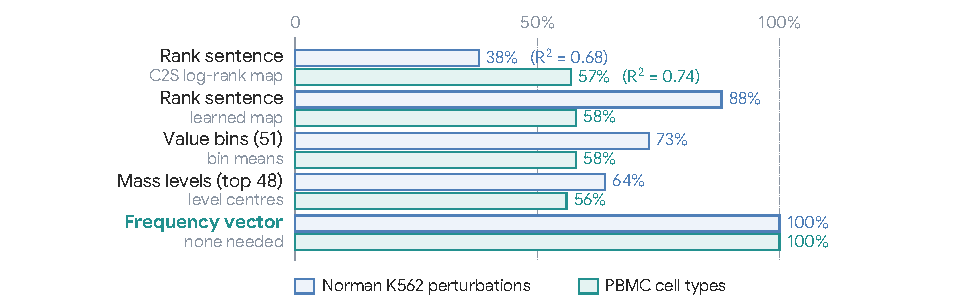
\includegraphics[width=\linewidth]{figs/fig3_representation.pdf}
\caption{\textbf{The likelihood a rank sentence loses depends on how it is decoded.} Real held-out test cells were rewritten in each representation and decoded back to gene frequencies; bars give the share of the likelihood gain of the cells' own frequency vectors over the reference (perturbed mean for Norman, cell-type mean for PBMC) that survives, all estimated from the same cells in the same way. The C2S log-rank map keeps $38\%$ on Norman although it reconstructs log expression with $R^2=0.68$, the criterion used to motivate rank sentences~\citep{levine2024cell2sentence}; a map learned on training cells keeps $88\%$. Shares from decoding real cells, not model results; the learned map was added after the test results.}
\label{fig:repr}
\end{figure}

\textbf{Where a sentence loses likelihood.} To separate the representation from the model, we rewrote the \emph{real} held-out cells of each unit in a representation, decoded them back to frequencies, and asked how much of the likelihood gain of the cells' own frequency vectors survives (Figure~\ref{fig:repr}). With the published log-rank map, the rank sentence reconstructs log expression well ($R^2=0.68$ on Norman, $0.74$ on PBMC), yet keeps only $38\%$ of the gain on Norman, against $73\%$ for value bins and $64\%$ for mass levels. A map learned on training cells, the mean frequency of each gene at each rank position, keeps $88\%$ from the same sentences ($90\%$ when the library size is also given). Most of the loss therefore lies in the map from ranks to counts rather than in the ranks themselves: the ordering of a K562 cell's genes carries most of its composition, but a sentence must be decoded, and the decoder determines how much survives, with about a tenth lost under every map we tried. On PBMC the representations do not separate ($56$--$58\%$ each), because cell types differ mostly in which genes are expressed. A generator that outputs the composition needs no such map, and its likelihood is defined by the model itself.

\subsection{The gain comes from the distribution output, not from the language model}\label{sec:lm}\label{sec:backbone}
\autoinput{auto_rev3/tab_e1.tex}
\textbf{Matched controls.} We compared \cad{} without a control cell against two controls, specified before they were run (Table~\ref{tab:e1}), with the same training cells, target, log-prior, softmax output, and scoring: the same language model \emph{frozen}, with only an MLP head trained on its last-token state; and a decoder with \emph{no language model}, in which a perturbation is the sum of learned embeddings of its genes (an unseen gene gets a zero embedding) followed by an MLP. On test, the decoder without a language model ties \cad{} in every stratum and for every seed (overall $-0.005$ nats per UMI, CI $-0.017$ to $+0.009$; seeds $1$ and $2$: $-0.007$ and $-0.003$) and on the downstream response ($r_{\mathrm{DE}}$ $-0.012$, CI $-0.042$ to $+0.016$), with $1.1$ million parameters trained in $10$ seconds. The frozen language model is worse ($+0.043$, CI $+0.025$ to $+0.060$; $r_{\mathrm{DE}}$ $-0.108$), most on pairs of seen genes ($+0.096$). On validation, with the Qwen backbone, the no-language-model decoder was $0.013$ nats worse (CI $0.000$ to $0.028$); by the rule fixed before these runs, which is evaluated on test, the likelihood gain over C2S and the perturbed mean comes from decoding the distribution directly, not from knowledge in the language model.

\textbf{Biological gene embeddings.} Giving every gene, including unseen ones, a frozen biological embedding does not help either (post hoc). GenePT embeddings of NCBI gene summaries~\citep{chen2024genept} are worse than learned embeddings overall ($+0.031$ against \cad{}, CI $+0.007$ to $+0.067$) and on unseen single genes ($+0.022$ against learned embeddings, CI $+0.005$ to $+0.040$), and co-expression embeddings from training cells tie \cad{} ($+0.006$, CI $-0.008$ to $+0.021$) with a lower $r_{\mathrm{DE}}$.

\textbf{Gene names and backbone.} Fine-tuning is what makes the language model as good a decoder of the condition as a purpose-built encoder; its added value is the interface, one prompt format for any state, which lets the same model generate cell types it has never seen (Section~\ref{sec:condgen}). Replacing gene symbols by opaque identifiers worsens the downstream response even on pairs of seen genes ($r_{\mathrm{DE}}$ $0.87$ against $0.89$; overall $0.69$ against $0.77$). Since an identity-only embedding without any text matches the model that reads real names, the names act as identifiers, and opaque tokens that share sub-words (GENE001, GENE002, \dots) blur them; on unseen single genes the names bring nothing measurable ($+0.007$ nats, CI $-0.022$ to $+0.030$), nor do NCBI gene summaries (validation). The backbone matters modestly: across three seeds, the C2S-initialized Gemma is $0.011$ to $0.012$ nats better than the general-purpose Qwen3.5-0.8B on both tasks, more than the seed spread ($0.001$ to $0.003$), without changing any ranking; LoRA ranks 8 to 64 give the same NLL.

\subsection{\cad{} matches additive composition downstream but shrinks target induction}\label{sec:pert}
\autoinput{auto_rev3/tab_norman_main.tex}
\textbf{Likelihood and realism (Table~\ref{tab:norman_main}).} Without a control cell, \cad{} is $0.104$ nats per UMI better than the perturbed mean (CI $0.071$ to $0.139$) and ties the additive baseline ($-0.009$, CI $-0.037$ to $+0.010$). Its generated cells are closer to real ones than additive cells (MMD $0.039$ against $0.052$; AUC $0.81$ against $0.86$), but not than those of the scGen-style shift, which moves each control cell individually. GEARS with default settings is $0.47$ nats above the perturbed mean after its regression output is mapped to frequencies (Appendix~\ref{app:val}); this measures that conversion as much as the model.

\autoinput{auto_rev3/tab_strata.tex}
\textbf{Downstream response, target gene set aside (Table~\ref{tab:strata}; post hoc).} CRISPRa raises its own target, so a model can look right on the target alone. With the perturbed genes removed, \cad{} reproduces the direction of $89\%$ of the top-20 downstream genes and ties additive on $r_{\mathrm{DE}}$ overall ($0.77$ against $0.77$; $+0.004$, CI $-0.033$ to $+0.040$) and in every stratum, and is better than scGen-style ($0.72$) and C2S ($0.56$). On the target genes themselves, it is \emph{worse} than additive on pairs (target error $0.51$ against $0.27$ with one unseen gene, $0.58$ against $0.39$ with both seen). The error is directional: the true induction of a target is about $1.7$ log units, additive composition copies it from the training single perturbation almost without bias ($+0.04$ to $+0.09$), and \cad{} under-predicts it by about $0.5$, shrinking a large gene-specific change toward the mean composition it learns a correction to (only $4$ of the $21$ unseen single targets are in the main panel, so this concerns pairs). The shrinkage is an output effect that a prior removes (post hoc): setting each target seen alone in training to its own training-single frequency, and multiplying unseen targets by the global induction factor, lowers \cad{}'s target error to $0.26$ and $0.29$, at or below additive, without changing its likelihood ($-0.011$ against additive, CI $-0.038$ to $+0.007$) or its downstream $r_{\mathrm{DE}}$. The negative-binomial head, which reweights genes by dispersion, does not (target error $0.63$ and $0.67$). Because a target gene carries little transcript mass, these changes move the NLL by less than $0.003$ nats; likelihood and target accuracy are separate properties and we report both.

\textbf{Genes never perturbed in training.} On the $21$ genes never perturbed in training, no learned model makes a gene-specific prediction: \cad{} ties the perturbed mean ($-0.006$, CI $-0.025$ to $+0.018$; $r_{\mathrm{DE}}$ $0.54$ against $0.51$), and the no-language-model decoder, $0.017$ nats better (CI $0.005$ to $0.028$), gives every unseen gene the same decoded empty state, a generic perturbation response; a split-half oracle lies $0.108$ nats below the perturbed mean (Appendix~\ref{app:kfold}). To score the targets themselves, we rebuilt the panel with every perturbed gene forced in, keeping the splits (Appendix~\ref{app:tp}; post hoc): on the $19$ unseen single genes whose target is then in the panel, \cad{}, the no-language-model decoder, and both embedding variants all predict almost no self-induction (target error $1.6$ to $1.7$ log units against $1.8$ for the perturbed mean; the target goes up in only $26$ to $42\%$ of predictions), whereas the one-factor target-induction baseline, which encodes only that CRISPRa raises its target, halves the error ($0.93$) and gets the direction right for $95\%$ of them.

\textbf{Worked examples (Figure~\ref{fig:example}).} For the median unseen gene, MAML2, its own induction is the largest change among its top-20 DE genes, and neither \cad{} nor any baseline predicts it: a decoder that has never seen the gene perturbed cannot infer this from its name. For the median pair of seen genes under the control residual, FOXA1+FOXL2, \cad{} reproduces the downstream program in direction (Pearson $0.87$ on the top-20 DE genes, against $0.83$ for additive) while compressing the largest changes, the same shrinkage as for target genes; and on the same fixed gene axis, each control cell yields its own distribution around the mean, which is how the per-cell model represents cell-to-cell variation.

\begin{figure}[!htb]
\centering
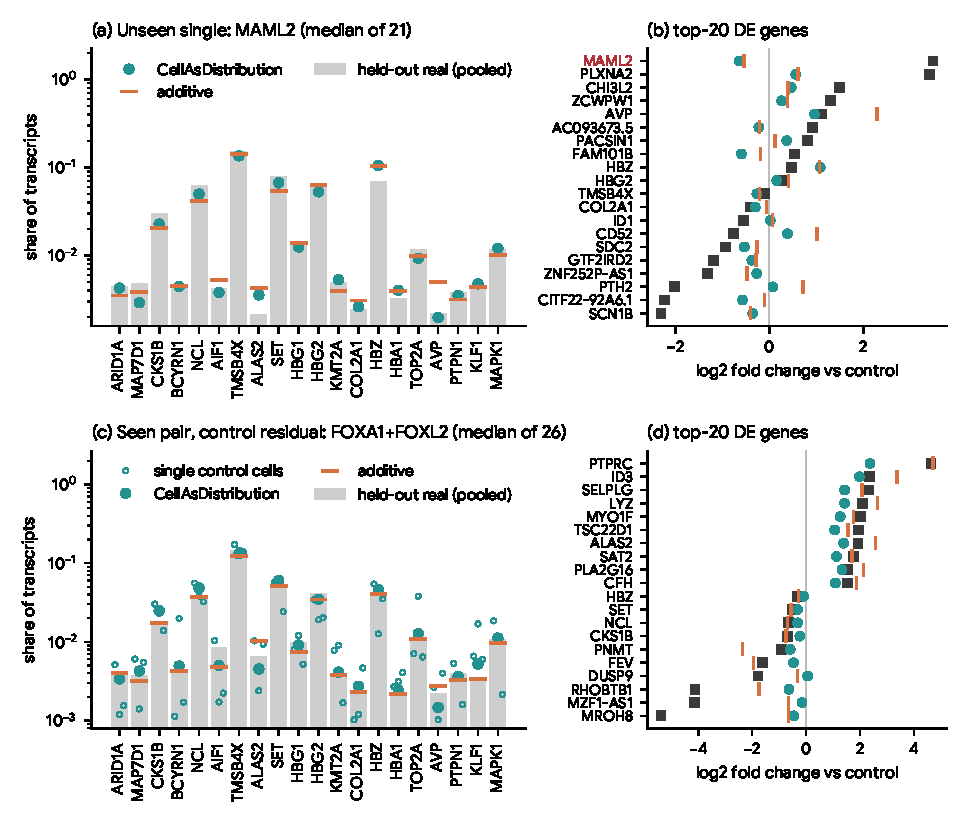
\includegraphics[width=0.92\linewidth]{figs/demo_main.pdf}
\caption{\textbf{What the decoder gets right and wrong, on two median test perturbations} (the unit with the median paired NLL difference to additive in its stratum, so not hand-picked; Norman test split, Gemma, seed 0). (a, c) The decoded distribution on a fixed gene axis: the $20$ panel genes with the highest mean frequency in training cells, in the order of the decision head's outputs and identical in both rows, so only the distribution changes. Grey: held-out real cells; teal: \cad{}; orange: additive composition; hollow teal: distributions decoded for three individual control cells. (b, d) Log fold change over the held-out control mean of the perturbation's top-20 DE genes (Welch $t$ on real cells), perturbed genes in red. (a, b) MAML2, never perturbed in training: no model predicts its self-induction; \cad{} and additive (here the perturbed mean) are both near the mean composition. (c, d) FOXA1+FOXL2, both genes seen alone in training, with the control cell as the log-prior: \cad{} recovers the direction of the downstream changes but compresses the largest ones, and each control cell gives a different distribution on the same genes.}
\label{fig:example}
\end{figure}

\subsection{Cell-to-cell variation enters through the control cell}\label{sec:residual}\label{sec:heads}
A single $q$ per perturbation leaves all cell-to-cell variation to the sampler. With the control cell as the log-prior ($b=\mathrm{smooth}(x_0)$, not written in the prompt), the cell NLL improves from $5.186$ to $5.129$ and the cells become more realistic (MMD $0.030$, AUC $0.79$), approaching scGen-style on MMD. Writing the control cell into the prompt instead loses this gain ($+0.019$ nats per UMI in cell NLL, CI $+0.012$ to $+0.027$). A version of the residual without a language model, in which the additive shift replaces the learned correction, reaches the same likelihood ($5.134$) but produces less realistic cells (MMD $+0.008$, AUC $+0.030$ relative to \cad{}). The residual has a cost: its downstream $r_{\mathrm{DE}}$ falls to $0.72$, below additive ($-0.046$, CI $-0.092$ to $-0.008$), because each control cell's own deviations enter the prediction.

\textbf{Distributional heads.} Two heads keep the single pass and the normalization of $q$ while modeling variation the flat softmax lacks (Appendix~\ref{app:heads}): a low-rank logistic-normal head, $q(c,z)$ along $16$ learned gene programs, lowers the cell NLL to $5.096$ without any control cell at the cost of the pooled NLL ($+0.062$); a negative-binomial head with per-gene dispersion improves the change correlation over all genes ($r_\Delta$ $+0.020$) at a small cost in NLL. Gene--gene correlations of generated cells on 100 variable genes are close to those of real cells for every method at this sequencing depth (Appendix~\ref{app:coexpr}).

\subsection{\cad{} reaches the type mean for known cell types and generates unseen ones from their names}\label{sec:condgen}
\autoinput{auto_rev3/tab_pbmc.tex}
\textbf{Known types (Table~\ref{tab:pbmc_main}).} As the remark of Section~\ref{sec:decoder} predicts, no model improves on the cell-type mean in likelihood on unseen donors: \cad{} is slightly worse ($+0.017$, CI $+0.001$ to $+0.036$), scVI and scANVI tie it, and on validation \cad{} gives the same NLL to four decimals for every LoRA rank and both backbones. Sample realism is decided by the source of cell-to-cell variation: scVI sampling from its own negative binomial reaches the lowest MMD and AUC ($0.92$), every frequency decoder relies on the shared sampler, and no generator is nearly indistinguishable from real cells of unseen donors (AUC $\ge0.92$).

\autoinput{auto_rev3/tab_zeroshot.tex}
\textbf{Unseen types (Table~\ref{tab:zeroshot}).} A model indexed by cell type cannot generate a type it has never seen; a decoder that reads the type's name can. In five leave-types-out folds over $19$ types, \cad{} with the Qwen backbone generates each held-out type from its name and Cell Ontology definition. It is $0.707$ nats per UMI better than the global mean (CI $0.545$ to $0.862$) and better than the nearest Cell Ontology type and the pooled Cell Ontology parents; it ties a string-matching baseline that copies the training type whose name shares the most words ($-0.058$, CI $-0.219$ to $+0.101$) but recovers the requested type far more often ($0.14$ against $0.02$). With the general-purpose Qwen backbone, the definition adds nothing beyond the name, and opaque identifiers remove the gain: that model generalizes by composing the words of type names. With the C2S-Scale-Gemma backbone, pretrained on cell sentences annotated with cell types (post hoc; same folds and settings), the name alone does better than string matching ($-0.216$, CI $-0.370$ to $-0.088$; $-0.865$ against the global mean) and recovers the requested type more often ($0.20$); definitions again add nothing, and opaque identifiers again fail. This is the one place in our study where pretrained knowledge helps, and it is knowledge of cell-type names learned from cell data: the pretraining corpus of C2S-Scale contains annotated immune cells, possibly including these types, so the gain may reflect exposure to them rather than inference from language.

\FloatBarrier
\section{Discussion and limitations}
Letting a decision language model answer with a gene distribution makes a language model a single-cell generator whose output is a cell's composition rather than a sentence about it. The interface has concrete consequences: generation costs one forward pass, the model's likelihood is defined without a reconstruction map, and every method can be compared on one proper score. The comparison with rank sentences shows why the last point matters: the same sentences keep $38\%$ or $88\%$ of the achievable likelihood depending on the map chosen to decode them, so a sentence model's quality cannot be separated from a post hoc choice, whereas a distribution is scored as produced.

Our controls are equally clear about what the language model does and does not do. On perturbations, a decoder of learned gene embeddings with the same output matches it, and neither a frozen language model nor biological gene embeddings do better, so the decision-native output, not language-model knowledge, carries the gain. For cell types, the language model is what makes unseen types reachable at all, and a backbone pretrained on annotated cell sentences reads their names better than string matching. The interface therefore separates two questions that sentence generation entangles: how a cell is represented and scored, which the distribution head settles, and what prior knowledge the encoder brings, which can then be measured.

A better gene distribution is not yet better biology, and our biological results draw a clear boundary. Where training contains the perturbed genes, the decoder matches additive composition on likelihood and on the downstream program, and generates more realistic cells; it shrinks the target's own induction, which an explicit prior corrects; and for genes never perturbed in training, none of the learned representations we tested (gene names, NCBI summaries, GenePT, or co-expression embeddings) predicts even the self-induction captured by a one-parameter biological prior. A categorical cell type caps any decoder at the type mean, while names let it generate unseen types. The output $q$ is a composition, not a probability of differential expression or of an intervention's success; a decision head trained on such events, with calibration measured on held-out perturbations, is the natural next step for the decision-native interface, together with richer states (donor, cell, and pathway context) and heads that model dispersion and covariance jointly.

\paragraph{Limitations.}
Our study is limited to one dataset per task, a fixed $2048$-gene panel, and CRISPRa perturbations; held-out control cells are not paired with perturbed cells, so cell NLL rewards covering cell states rather than predicting individual counterfactuals; GEARS was evaluated with default settings, and CPA as well as transport and flow models were omitted because they do not output a distribution over a fixed gene list; the C2S-Scale pretraining corpus may contain the PBMC cell types, so the Gemma zero-shot result is not a clean test of generalization; and the downstream, target, target-prior, add-on-panel, gene-embedding, Gemma zero-shot, co-expression, and learned-rank-map analyses were added after the test results (Appendix~\ref{app:protocol}).

\paragraph{Code availability.} Code, held-out unit lists, run scripts, and table-generation scripts are available with a README at \url{https://github.com/kagtgi/CellAsDistribution}.
\paragraph{AI use statement.} Code, experiments, tables, figures, and a first draft of this text were produced with assistance from Claude (Anthropic); the authors reviewed all content and are responsible for it.

{\interlinepenalty=10000
\bibliographystyle{unsrtnat}
\bibliography{refs}}
